% 
% Annual Cognitive Science Conference
% Sample LaTeX Paper -- Proceedings Format
% 

% Original : Ashwin Ram (ashwin@cc.gatech.edu)       04/01/1994
% Modified : Johanna Moore (jmoore@cs.pitt.edu)      03/17/1995
% Modified : David Noelle (noelle@ucsd.edu)          03/15/1996
% Modified : Pat Langley (langley@cs.stanford.edu)   01/26/1997
% Latex2e corrections by Ramin Charles Nakisa        01/28/1997 
% Modified : Tina Eliassi-Rad (eliassi@cs.wisc.edu)  01/31/1998
% Modified : Trisha Yannuzzi (trisha@ircs.upenn.edu) 12/28/1999 (in process)
% Modified : Mary Ellen Foster (M.E.Foster@ed.ac.uk) 12/11/2000
% Modified : Ken Forbus                              01/23/2004
% Modified : Eli M. Silk (esilk@pitt.edu)            05/24/2005
% Modified: Niels Taatgen (taatgen@cmu.edu) 10/24/2006

%% Change ``a4paper'' in the following line to ``letterpaper'' if you are
%% producing a letter-format document.

\documentclass{article} % For LaTeX2e

\usepackage{nips12submit_e,times}
\usepackage{pslatex}
\usepackage{amsmath}
\usepackage{amsfonts}
\usepackage{latexsym}
\usepackage{amssymb}
\usepackage{graphicx}
\usepackage{xspace}
\usepackage{multirow}
\usepackage{array}
\usepackage{caption}
\usepackage{subcaption}
\usepackage{float}
\usepackage[numbers]{natbib}

\newcommand{\dictionary}{\ensuremath{\mathcal{D}}\xspace}

\title{Halo, Hyperbole, and the Pragmatic \\ Interpretation of Numbers}
 
\author{
Jean Y. Wu \\
Symbolic Systems Program\\
Stanford University\\
Stanford, CA 94305 \\
\texttt{jeaneis@stanford.edu} \\
\And
Justine T. Kao \\
Department of Psychology\\
Stanford University \\
Stanford, CA 94305 \\
\texttt{justinek@stanford.edu} \\
\AND
Leon Bergen \\
Department of Brain and Cognitive Sciences\\
Massachusetts Institute of Technology \\
Cambridge, MA 02138\\
\texttt{bergen@mit.edu} \\
\And
Noah D. Goodman \\
Department of Psychology\\
Stanford University \\ 
Stanford, CA 94305\\
\texttt{ngoodman@stanford.edu} \\
}


\begin{document}

\maketitle

\begin{abstract}
Numbers are interpreted flexibly in everyday language: imprecision, exaggeration, and hyperbole are everywhere. We propose a computational model of the pragmatic interpretation of numbers, building upon recent models of pragmatics as rational inference. We assume that speaker and listener perform a social inference regarding the intended meaning, precision, and affective subtext of a numerical utterance. This model predicts \emph{pragmatic halo}, \emph{hyperbole}, and their interaction. We demonstrate that the model accurately predicts the qualitative effects of human interpretation of number words in five real-world domains.
%We hypothesize that hyperbole allows speakers to minimize the cost of an utterance while maximizing the message conveyed. Meanwhile, the listener infers additional information embedded in the utterance, namely the true state of the world in addition to the speaker's opinion. We investigate these predictions using a Bayesian computational model and a behavioral experiment and show that our model is able to exhibit the effects of pragmatic halo and hyperbole as well as their interaction.
\textbf{Keywords:} 
Number interpretation, hyperbole, pragmatic halo, pragmatics, Bayesian model
\end{abstract}


\section{Introduction}

The meanings of numbers are usually thought to be fixed and precise. In mathematics, the number $30$ has a precise meaning that clearly distinguishes it from $32$ and $1000$. In everyday language, however, numbers are treated much more flexibly: people do not always mean what they say when using number words. In this paper we examine the pragmatic interpretation of number words using formal models and behavioral experiments.
%the kinds of inference mechanisms that people utilize in order to identify when a number is not intended to be interpreted literally. 
In particular, we explore the phenomena of \emph{pragmatic halo} and \emph{hyperbole.} Halo refers to imprecise use of number words (for instance, ``I'll be there in 30 minutes'' means \emph{about} 30 minutes); hyperbole refers to the use of exaggeration to convey affective subtext (for instance, ``I waited for a million hours'' means roughly ``I waited for a while and I didn't like it'').
Building on recent models of pragmatics as rational inference by a speaker and listener about each other, we propose a computational model that captures both halo and hyperbole effects, as well as their interaction.

Pragmatic halo refers to the tendency toward imprecise interpretation of simple number expressions coupled with the precise interpretation of complex number expressions \cite{lasersohn1999pragmatic}. Suppose a friend tells you: ``I will be there in $30$ minutes." The number $30$ can be interpreted as meaning somewhere within a broad range, say from $25$ to $40$ minutes. On the other hand, if your friend says: ``I will be there in $32$ minutes," it is more likely that you would interpret the number to mean exactly $32$. 
%The intuition behind this is that if your friend intended to convey the meaning of ``somewhere around $32$", she would have uttered $30$ instead, because $30$ conveys the same meaning and is less effortful to utter. 
Krifka \cite{krifka2007approximate} described how this pragmatic halo effect can be explained under the assumption that speakers prefer number expressions that are shorter and less costly to utter. Listeners will then favor approximate interpretations of round numbers even if there is no general bias for approximate interpretations. Bastiaanse \cite{bastiaanse2011rationality} further argued that interpreting round numbers as approximate is a rational choice, as can be formalized via game theory \cite{jager2008game}. 
%note: this cite should be:  http://www.sfs.uni-tuebingen.de/~gjaeger/publications/hskArticleGJ-2011.pdf
Here we capture these arguments within a Bayesian framework for pragmatic inference: if number words could be interpreted precisely or approximately, and some number words are more costly than others, we show that a rational listener will interpret the more costly number words as more precise.
%Here we refer to this effect as the \emph{pragmatic halo}, where certain numbers tend to be interpreted with less precision than others. For example, the possible interpretations of the number $30$ is a distribution centered around $30$.

Not only can numbers be used loosely, they can also be used hyperbolically.
Suppose you overhear a student saying, ``It takes 30 minutes to scroll down that professor's list of publications!" Given that it is very unlikely for the literal meaning of the utterance to be true, the number $30$ in this utterance is likely to be interpreted as much less than 30 minutes, though still greater than average. Moreover, an affective subtext is likely to be conveyed: the list of publications is strikingly long.
Hyperbolic utterances often express important interpersonal meaning beyond the literal meaning of the statement, and successful interpretation of such expressions hinges on the listener's ability to infer the speaker's intentions \cite{mccarthy2004there, gibbs2000irony, cano2003risk}. Previous work has focused on cues for verbal irony and exaggeration, such as a slow speaking rate, heavy stress, nasalization, and interjections \cite{kreuz1995two, kreuz2007lexical}. Although lexical and prosodic information has been shown to be important for human and machine detection of hyperbole \cite{davidov2010semi, reyes2011mining, van2007algorithm}, we argue that common prior knowledge about the relevant topic
%the distribution of numerical values associated with the relevant topic 
also plays an important role in identification and interpretation of hyperbolic statements. That is, part of what makes a statement likely to receive a hyperbolic interpretation is that both speaker and listener know the literal meaning is very unlikely. 
While a publication list that takes thirty minutes to scroll is very unlikely, waiting for a friend for thirty minutes is not; correspondingly, ``30 minutes'' is likely to be interpreted as hyperbolic for scrolling times, but as approximately literal for waiting times.
%For example, suppose that the cost of a tall latte at Starbucks is always $2.75$ dollars, and suppose someone who went to Starbucks every day told you, ``That Starbucks tall latte cost, like, two dollars and seventy-five cents!" Even if the statement was uttered with many interjections, a slow speaking rate, heavy stress, and nasalization, it would be difficult to interpret the utterance as being hyperbolic, because the distribution of numerical values associated with Starbucks tall lattes is a single value at $2.75$. As a result, we propose that the statistical properties and distributions of numbers in the natural world should serve as a major cue for hyperbole detection.


%%FIXME: this paragraph is kind of vague.
%What additional information do hyperbolic utterances convey beyond their literal counterparts, and how does a listener recover this information? We hypothesize that when people utter a hyperbolic statement, they express an opinion in addition to a description of the state of the world. Hyperbole allows speakers to minimize the cost of an utterance while maximizing the message conveyed. Meanwhile, the listener should be able to infer the additional information embedded in the utterance, namely the true state of the world in addition to the opinion. We will investigate these predictions using a Bayesian computational model and a behavioral experiment. 

In this paper we describe how these non-literal uses of number terms can be explained as effects of probabilistic inference over recursive social models.
We build on a traditional approach within linguistics, which views communication as an interaction between rational, cooperative agents \cite{grice1975, clark1996using}. 
%clark, ``Using language''
The speaker in a conversation has a message to communicate, and her goal is for the listener to understand this message. The listener's goal is to infer the intended meaning of the message from the speaker's utterances. The listener performs Bayesian inference to infer the intended meaning, while the speaker is a rational planner who takes into account how the listener will interpret each utterance. 
Recent work \cite{frankgoodmanscience, goodmanstuhlmueller} has shown that a simple formal model of this interaction is able to quantitatively explain human pragmatic reasoning. We will be working with extensions of this model, in which the speaker and listener recursively reason about one another \cite{jager2009pragmatic, bergen2012, franke2009interpretation}. Here, the listener reasons about a speaker who optimizes informativeness of her utterances; the speaker optimizes assuming that the listener is reasoning in this way about the speaker; and so on. These models of recursive social reasoning are closely related to signaling games \cite{cho1987signaling, chen2008selecting}. In the case of number words, we will show how this framework can be applied to capture pragmatic halo, hyperbole, and their interactions.

%The rest of the paper is organized as follows. Section 2 provides an overview of previous work on hyperbole and pragmatics. Section 3 describes the computational model and its predictions. Section 4 describes the behavioral experiment and results. Section 5 compares the model results to the behavioral data and discusses implications. Section 6 proposes directions for future work.
%%%%

\section{Model}

We begin by describing a version of the framework that is able to capture the basic pragmatic halo and exaggeration effects.
%: more complex utterances are interpreted as being more precise. 
Each listener will be associated with a dictionary $\dictionary$, which specifies the literal meaning of each possible utterance: a function assigning a probability to each meaning. (The dictionary can thus be seen as an undirected probabilistic model relating words to meanings.) The listener's dictionary determines a \emph{literal interpretation} of the utterance. We will assume that meanings are integers in a set $\mathcal{I}$, and, with a slight abuse of notation, that utterances come from the same set. For each utterance $u$, the dictionary entry $\dictionary_u$ will be proportional to a one-dimensional normal distribution $f(x;u,\sigma^2)$ of mean $u$---that is the word ``u'' means approximately $u$. After hearing the utterance $u$, the listener $L_0$ updates his prior distribution $P$ over meanings \emph{m} by conditioning $P$ on the dictionary entry for $u$:
\begin{align}\label{eq:literallistener}
L_0(m | u, \dictionary) &\propto \dictionary_u(m)P(m) \\
&\propto f(m;u,\sigma^2)P(m).
\end{align}
%For modeling pragmatic halo, we can assume that the prior $P$ is uniform over meanings.

This literal listener provides the base case for recursive social reasoning between the speaker and listener. In general, the speaker $S_n$ is assumed to be a rational planner who is optimizing the probability that her intended meaning \emph{m} will be understood by the listener $L_n$ while minimizing the cost of the utterance. The listener $L_n$ performs Bayesian inference to guess the intended meaning given prior $P$ and his internal model of the speaker $S_{n-1}$.

The speaker $S_n$ chooses utterances according to a softmax decision rule that describes an approximately rational planner \cite{sutton1998reinforcement}:
\begin{equation}\label{eq:speakerprob}
S_n(u | m,\dictionary) \propto e^{\lambda U_n(u | m,\dictionary)},
\end{equation}
where the constant $\lambda$ captures the degree of optimality of the speaker. 
The speaker wants to minimize both the cost $c(u)$ of the utterance and the surprisal of the intended meaning $m$, so the utility function $U_n$ is defined by:
\begin{equation}\label{eq:speakerutility}
U_n(u | m, \dictionary) = \log (L_{n}(m | u, \dictionary)) - c(u),
\end{equation}
which combined with equation \ref{eq:speakerprob} leads to:
\begin{equation}\label{eq:speakersimplified}
S_n(u | m, \dictionary) \propto (L_{n}(m | u,\dictionary)e^{-c(u)}) ^\lambda.
\end{equation}

The speaker $S_0$ reasons about the literal listener $L_0$, and assumes that this listener shares her dictionary $\dictionary$. However, in general the listener will be uncertain about the dictionary being used by the speaker, which we call \emph{lexical uncertainty} \cite{bergen2012}. This lexical uncertainty provides room for context-specific uses of certain words. To determine the speaker's intended meaning, the listener will therefore marginalize over the possible dictionaries being used:
\begin{equation}\label{eq:listenerdict}
L_n(m|u,\dictionary) \propto \sum_{\dictionary_i }P(m)P(\dictionary_i)S_{n-1}(u | m,\dictionary_i).
\end{equation}
Substituting equation \ref{eq:listenerdict} into equation \ref{eq:speakersimplified} we can see that the dictionary $\dictionary$ plays no role in the reasoning of the listener $L_n(\cdot|u,\dictionary)$ or the speaker $S_n(\cdot| m, \dictionary)$ for $n>0$. This leads us to:
\begin{equation}
  L_n(m | u) :=  L_n(m | u, \dictionary) \text{ ~~~~~ if $n > 0$}
\end{equation}
\begin{equation}
  S_n(u | m) :=  S_n(u | m, \dictionary) \text{ ~~~~~ if $n > 0$.}
\end{equation}

We assume in this paper that the prior probability on dictionaries $P(\dictionary_i)$ is uniformly distributed across a set of possible dictionaries. 
Initially, the dictionary $\dictionary$ simply determines the standard deviation $\sigma_u$ associated with each number utterance $u$, therefore specifying how precisely each utterance will be interpreted by the literal listener. Lexical uncertainty thus represents uncertainty about how precisely the speaker believes her utterances will be interpreted. 


\subsection{Pragmatic halo}

This model predicts the pragmatic halo effect. For now we may assume that $P(m)$ is uniform over meanings, but that $c(u)$ varies---some utterances are more costly than others (whether this cost comes from length, frequency, or other factors).

To understand why the model predicts that more complex utterances will be interpreted more precisely, we will look at the simplest possible example of this effect (Figure \ref{fig:model}a). Suppose there are two possible meanings, numbers \emph{1} and \emph{2}, and two possible utterances, number words ``one" and ``two." Suppose that ``two" is much more expensive than ``one." First suppose the speaker wants to communicate \emph{1}. In this case, the speaker will almost never choose to communicate using the utterance ``two." The utterance ``two" is more expensive than utterance ``one," and its literal meaning is strictly farther away from the speaker's intended meaning, implying that it receives a small likelihood from equation \ref{eq:speakersimplified}. Because utterance ``one" is cheaper and closer to the intended meaning, it will receive most of the probability mass allocated by this equation.

In contrast, suppose the speaker wants to communicate \emph{2}. In this case the two utterances are more evenly balanced, with two factors pulling against each other in equation \ref{eq:speakersimplified}. The literal meaning of utterance ``two" is closer to the intended meaning, but utterance ``one" is cheaper. The utterance ``one" could therefore be used by speakers trying to communicate either meaning, while the utterance ``two" will only be used by speakers trying to communicate \emph{2}. When the listener uses equation \ref{eq:listenerdict} to infer the speaker's intended meaning, he will reason about the likelihood of the utterances being produced by each speaker, and infer that the utterance ``two" means \emph{2}, while the utterance ``one"  is ambiguous between the two meanings. It follows that ``two" will be assigned a more precise meaning which peaked on \emph{2}.  Figure \ref{fig:model}a illustrates the pragmatic effect that our model produces. Utterance ``two" is assigned a higher cost than utterance ``one", and the prior probabilities of the meanings \emph{1} and \emph{2} are identical. After eight levels of recursion between the listener and speaker models, the listener assigns similar probabilities for meanings \emph{1} and \emph{2} to the utterance ``one," and a probability of $1$ for meaning \emph{2} to the more expensive utterance ``two." Our model thus interprets the cheaper utterance loosely and the expensive utterance precisely---this is the pragmatic halo if we assume cost is related to ``roundness'' of the numbers.


\subsection{Exaggeration}

\begin{figure}[t]
        \begin{subfigure}[t]{0.33\textwidth}
                \centering
                \caption{Pragmatic Halo}
		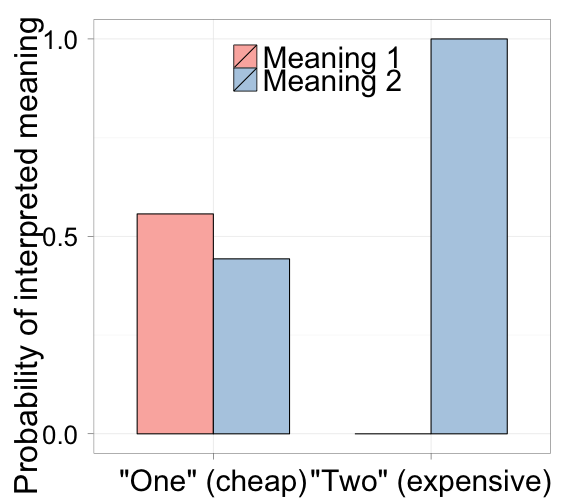
\includegraphics[width=\textwidth]{model_halo.png}
		
	\end{subfigure}
        \begin{subfigure}[t]{0.33\textwidth}
                \centering
                \caption{Exaggeration}
                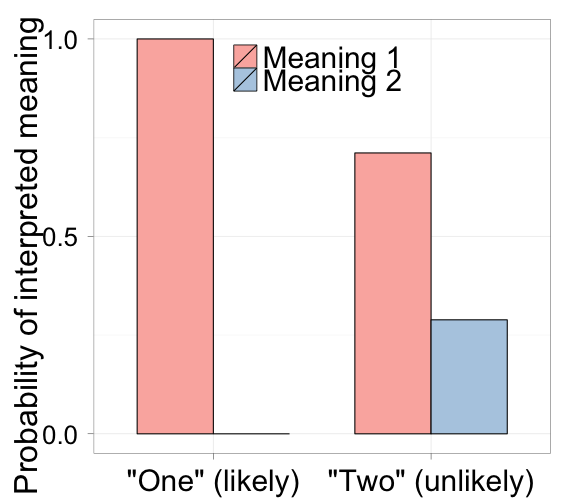
\includegraphics[width=\textwidth]{model_exagg.png}
		
	\end{subfigure}
	\begin{subfigure}[t]{0.33\textwidth}
                \centering
                \caption{Affect}
                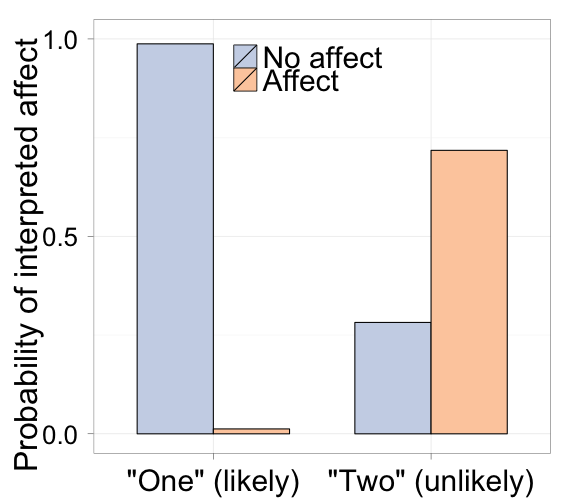
\includegraphics[width=\textwidth]{model_valence.png}
		
	\end{subfigure}
	\caption{Halo and hyperbole effects in the model's interpretation of utterances ``one" and ``two". Possible meanings are the numbers 1 and 2 (a, b) and affective subtext (c).}
	\label{fig:model}
\end{figure}

We now turn to the effect of the prior distribution over meanings, $P(m)$, and pragmatic exaggeration, i.e. the non-literal interpretation of utterances with extreme meanings. 
%Rather than cost, exaggeration is driven by the prior distribution over meanings. 
Pragmatic halo results from matched prior probabilities but different utterance costs; we will show that exaggeration is the pragmatic effect that results from matched costs but differing prior probabilities. 
Hence, we set the cost of all utterances $c(u)=0$, and set the prior distribution over meanings $P$ to be a unimodal distribution over the numbers $\mathcal I$. 

Given these assumptions, the model predicts that utterances with unlikely literal meanings will have their interpretations shifted towards the prior, while utterances with likely meanings will be interpreted literally (Figure \ref{fig:model}b). To illustrate this, we again consider an example with two meanings, \emph{1} and \emph{2}, and two utterances, ``one" and ``two." Suppose that the meaning \emph{1} is much more likely \emph{a priori} than \emph{2}. If the dictionary entry $\dictionary_{\text{``two"}}$ for the utterance ``two" is vague, then the literal listener in equation \ref{eq:literallistener} will revert to his prior and interpret this utterance as likely meaning \emph{1}. In contrast, the literal listener will never interpret ``one" as meaning \emph{2}: whether the dictionary entry for $\dictionary_{\text{``one"}}$ is vague or precise, the listener's prior will bias him towards interpreting the utterance as meaning \emph{1}. It follows that when the speaker reasons about the listener and chooses an utterance according to equation \ref{eq:speakersimplified}, she will sometimes use the utterance ``two" to convey the meaning \emph{1}, but will never use the utterance ``one" to convey the meaning \emph{2}. Thus the utterance ``two" may be used by speakers intending either meaning, and therefore may be interpreted as exaggerated, while the utterance ``one" will only be used by speakers intending meaning \emph{1}, and will be interpreted literally. That is, because $2$ is an unlikely meaning, the word ``two'' is likely to be used loosely. Figure \ref{fig:model}b illustrates the exaggeration effect that our model produces. After eight levels of recursion between the listener and speaker models, the listener assigns a probability of $1$ for meaning \emph{1} to utterance ``one." However, it assigns a higher probability of meaning \emph{1} to utterance ``two" as well, even though the literal meaning of ``two" is \emph{2}. Our model thus interprets the utterance whose literal meaning is highly unlikely as exaggerated and as lower than the literal meaning.

\subsection{Affect and subtext}

How can we capture the subtext of a hyperbolic statement? Hyperbole is similar to exaggeration, except that additional information about the \emph{affect} of the meaning is conveyed. Affect is a second dimension of meaning, separate from the number value. If $A$ is the set of possible affects, then the set of possible meanings $M$ is given by:
\begin{equation}
M = {\mathcal I} \times A.
\end{equation}

We extend the model to be compatible with meanings that consist of number-affect pairs. The dictionary entry $\dictionary_u$ for an utterance $u$ now consists of a Gaussian centered around $u$ as before, as well as a truth function $T_u:A\rightarrow \{0,1\}$ that determines which affects are compatible with $u$. The truth function $T_u$ will be determined by the context. This means that in some contexts, an utterance $u$ will convey a negative affect along with its number meaning; in other contexts it will pick out a positive affect; and in still others it will be compatible with any affect. We may modify equation \ref{eq:literallistener} so that the literal listener is now defined by:
\begin{align}\label{eq:affectliteral}
L_0((k,a) | u, \dictionary) &\propto \dictionary_u(k,a)P(k,a) \\
&\propto f(k;u,\sigma^2)T_u(a)P(k)P(a),
\end{align}
where $k$ is the number that the speaker wants to communicate, $a$ is the affect, and we assume for simplicity that number and affect are independent under the prior. 
The rest of the model is extended in a similar manner. Lexical uncertainty now means that the listener is uncertain about which truth function is associated with each utterance $u$. This means that while speakers may believe that a specific affect is part of the literal meaning of their utterance, listeners are uncertain about these beliefs. Importantly, the meanings cary no \emph{a priori} content about affect: in expectation, each utterance is uniform over the affect dimension. 
%We note that there are now many more possible dictionaries: each utterance is assigned both a standard deviation and a truth function, and there are $2^{|A|}$ truth functions on affects. 

We will now illustrate how this model predicts hyperbolic interpretations of extreme utterances (Figure \ref{fig:model}c). We assume that there are two number meanings, \emph{1} and \emph{2}, and two affects, \emph{neutral} and \emph{negative}, so that there are four pairings of numbers and affects. We assume that \emph{1} is more likely than \emph{2}, and \emph{neutral} is more likely than \emph{negative}. There are two utterances, ``one" and ``two." If the speaker wants to communicate \emph{1}-\emph{neutral}, she is likely to succeed by saying ``one" whether its dictionary entry $\dictionary_{\text{``one"}}$ is vague or precise: as long as the dictionary entry $\dictionary_{\text{``one"}}$ is compatible with this meaning, the literal listener in equation \ref{eq:affectliteral} will be biased towards it. This speaker will therefore assign small probability to the utterance ``two," which is less likely to be interpreted correctly. On the other hand, there are two moderately likely meanings that may lead the speaker to say ``two": \emph{2}-\emph{neutral} and \emph{1}-\emph{negative}. It is clear why the speaker would say ``two" to communicate the first meaning \emph{2}-\emph{neutral}. For the second meaning, \emph{1}-\emph{negative}, the speaker may use the utterance ``two" if she believes that the dictionary entry  $\dictionary_{\text{``two"}}$ has a vague number meaning (and is therefore compatible with meaning \emph{1}) and that it uniquely picks out the negative affect. Because the speaker may use ``two" to communicate \emph{1}-\emph{negative}, it provides evidence to the listener in equation \ref{eq:listenerdict}, who is reasoning about the speaker, that this meaning was intended. This is the hyperbolic interpretation of the utterance ``two." Figure \ref{fig:model}c illustrates the effect of subtext that our model produces. After eight levels of recursion between the listener and speaker models, the listener assigns no affective information to utterance ``one," but assigns a high probability of affect to utterance ``two." Our model thus interprets the utterance with the unlikely literal meaning as imprecise and conveying an affective subtext.

%\subsection{The complete model}


Our final model combines the elements of the previous models. It is intended to simultaneously capture three effects: pragmatic halo, the interpretation of extreme utterances as exaggerated, and the interpretation of exaggerated utterances as hyperbolic. This model will allow the costs of utterances to vary, as in the model of pragmatic halo; allow prior probabilities of meanings to vary, as in the model of exaggeration; and introduce affects into the meaning, as in the model of hyperbole. Formally, the model will be identical to the model of hyperbole, except that we allow for utterance costs $c(u) > 0$. In addition to the effects already described, the complete model shows interactions. For instance, pragmatic halo is more extreme for unlikely utterances. We will describe and discuss the behavior of the complete model in comparison with results from our behavioral experiment (Figure 3).




\section{Experiment}

We conducted a behavioral experiment to test whether humans' interpretation of number words can be explained using the model described above. We tested the model on five different scenarios. In each scenario, a speaker makes an utterance that contains a numerical value conveying information about a particular item or state of the world, for example, the price of a textbook or the temperature outside. Subjects are then asked to interpret the numerical expression. Critically, by varying the prior probability of the number and whether it is round, we can explore factors leading to non-literal interpretation.

\subsection{Participants, Materials, and Methods}

We recruited $220$ subjects located in the United States through Amazon Mechanical Turk. (We excluded responses from $4$ non-native English speakers and $1$ response that contained an obvious typo.) Each subject read five short scenarios in random order regarding the following five domains: the number of minutes a bus is behind schedule, the price of a college textbook, the price of a parking ticket, the number of pages in a reading, and the weather temperature (in degrees Fahrenheit). We selected these domains because we believe people have reliable intuitions about the true distributions of such values, and also because people are likely to exaggerate and express opinions about these issues. Eight possible number values, $X$, were systematically chosen for each scenario. These values consisted of four pairs of two numbers. Each pair contained one round number (e.g. $100$) and a neighboring number that cannot be evenly divided by 10 (e.g. $102$). These neighboring non-round numbers also contain more syllables than their ``rounder" counterparts and are presumably more difficult to utter. The first value pair is close to the mean of the underlying distribution; the second and third value pair are moderately close to the mean; and the fourth value pair is very far from the mean. We chose these values in order to best compare the various effects that we wish to examine as well as how these effects interact. Each scenario was structured in a similar manner, and each subject saw only one of the $8$ possible values. Table 1 shows an example of the textbook scenario (remaining  scenarios are described in SI).


\begin{table}[h]
\begin{tabular}{| p{0.15cm}  p{8.15cm}| p{0.15cm}p{4cm} |}\hline
\multicolumn{2}{|c|}{\textbf{Scenario}} & \multicolumn{2}{c|}{\textbf{Values for X}} \\\hline
\multicolumn{2}{|l|}{Ann and Bob are friends. They are taking the same class.} & \multicolumn{2}{l|}{[$100$, $102$, $150$, $152$,}\\
\multicolumn{2}{|l|}{\textbf{Ann:} ``How much did the textbook cost you?"} & \multicolumn{2}{l|}{$200$, $202$, $1000$, $1012$]}\\
\multicolumn{2}{|l|}{\textbf{Bob:} ``\{X\} dollars."} & \multicolumn{2}{l|}{}\\\hline
\multicolumn{2}{|c|}{\textbf{Questions}} & \multicolumn{2}{c|}{\textbf{Responses}} \\\hline
(1) & Was Bob being literal about the cost of the textbook, & (1) &[Literal / Exaggerating] \\
 & or was he exaggerating? & (2) & [Free response] \\
(2) & How much do you think the textbook actually cost? & (3) & [Likert scale] \\
(3) & How negative does Bob feel about the cost of the textbook? & (4) & [Exactly \{X\} dollars / \\
(4) & What is Bob most likely trying to communicate by saying  ``\{X\} dollars"? & & Approximately \{X\} dollars / The textbook is expensive and Bob is not happy.]\\\hline
\end{tabular}
\caption{Example scenario of textbook costs.}
\label{tab:myfirsttable}
\end{table}


\subsection{Results}

% halo and exaggeration



Based on our model of pragmatic interpretation for numbers, we predicted that subjects' responses would exhibit the following phenomena. First, round numbers will be interpreted less literally. Second, less likely numbers will be interpreted non-literally and as closer to the mean. Third, exaggerated utterances will be interpreted as conveying stronger affect. Furthermore, there will be an interaction among these three effects, such that non-round numbers closer to the mean will be interpreted as the most precise and convey the least affect, while round numbers farther from the mean will be interpreted as the most exaggerated and will convey the most affect.

Overall results for three scenarios, with comparable model predictions, are shown in Figure \ref{fig:results} (remaining data are presented in SI). Before considering the full results, we explore halo and exaggeration effects. As shown in Figure \ref{fig:effects}, the proportion of subjects who interpreted an utterance literally varies as a function of the ``roundness" of the uttered value as well as the distance between the uttered value and the mean of the underlying distribution. To examine the pragmatic halo effect, we compared the precision of subjects' interpretation of round versus non-round numbers.
An interpretation is considered precise if it is identical to the uttered number. Figure \ref{fig:effects}a shows that round numbers are less likely to be interpreted exactly. 
%In other words, non-round numbers tend to invite a literal and precise interpretation. 
To examine the effect of prior probability on interpretation we compared exaggeration among the non-round numbers, considering an  interpretation exaggerated if it is lower than the literal value. Figure \ref{fig:effects}b shows that subjects are more likely to judge an utterance as exaggeration when the literal meaning of the numerical value becomes less likely in the particular domain under discussion. 

%For instance, when prompting subjects to a temperature of 107 degrees Fahrenheit, they judged it as exaggeration because it is unlikely that the weather gets that high in the United States, from which these subjects were recruited.

% exaggeration and affect (should we still add a plot that just has affect?)
% add something about how affect is computed: median split ( > 5 is affect).

%We then analyzed the relationship between exaggeration and speaker's affect. The graphs in Figure 3 show how each utterance is interpreted and illustrate the relationship between uttered values and their probability of being perceived to convey affect. 
To compare the full model with our behavioral results, we took the set $\mathcal I$ of meanings and utterances to be the eight values that subjects saw in each scenario. Because the prior distribution in each domain is roughly unimodal with mode at the lowest number considered, but the variance and the heaviness of the tail vary between domains, we model the prior distribution as geometric plus constant:
$P(m)\propto b^{m} + c$. Parameters for the priors and cost of utterances are described in Figure \ref{fig:results}.
%A small value of $c$ indicates that the listener is confident that the probability of extreme values is low in that particular domain, while a high value indicates that the listener still reserves significant mass to the prior probability of extreme values. 
We use the textbook scenario to illustrate. Our model interprets the utterance ``100" as most likely to mean $100$ without affective information. Since the model of the listener assumes that the speaker provides the most informative utterance, the model similarly interprets other numbers that have fairly high prior probabilities as literal. As the literal meaning of the utterance becomes less likely, the model begins to interpret the utterance as an exaggeration. This effect interacts with the pragmatic halo, such that the costlier utterances ``202" and ``1012" are not interpreted hyperbolically, while the less costly utterance ``1000" is interpreted as a value closer to the mean that carries affective information. These results from our model capture the patterns in our human data (Figure \ref{fig:results}b). 

%We now discuss ways in which differences across scenarios can be modeled by adjusting the prior distribution of meanings. 
The strength of the priors associated with the values in each scenario affects the values at which the probability of perceived exaggeration increases---that is the tendency to interpret a number as hyperbole depends on (common knowledge of) the statistics of the underlying domain. People have extensive experience with weather temperatures and likely know that the probability of the temperature being $150$ F is close to $0$. In other words, the prior distribution of weather temperatures drops off sharply after a certain value and has a very thin tail. Figure \ref{fig:results}d shows that people no longer interpret utterances above ``150" as literal. Adjusting the prior distribution in our model appropriately results in a similar abrupt transition.  On the other hand, subjects have weak prior knowledge about the probability of extreme quantities of reading for a class. Figure \ref{fig:results}f shows that even for utterances with extremely high values such as ``1018," a significant proportion of subjects still make literal interpretations (note, however, that due to the pragmatic halo effect, subjects do not interpret ``1000" as literal). This behavior can also be captured by setting the prior in our model to have a heavier tail. Figure \ref{fig:results}e shows that the model assigns significant probability to the literal meaning of ``1018" and demonstrates a pragmatic halo effect similar to that observed in the human data, such that the literal interpretation of non-round numbers is more likely than the literal interpretation of their neighboring round counterparts.

\section{Discussion and Future Directions}

%Despite having highly standard literal meanings, numbers are often used non-literally in everyday language. 
Our behavioral results show that people often interpret numerical expressions in imprecise or non-literal ways, even in the absence of phonological cues. However, there are complex patterns in this non-literal usage: hyperbole depends on prior probability, conveys affective subtext, and interacts with the halo of round numbers.
Building upon recent theoretical work, our computational model shows that rational recursive reasoning between speaker and listener can capture these effects of pragmatic halo and hyperbole. Our model introduces an ``affect" dimension to language interpretation, such that hyperbolic utterances efficiently convey information regarding the speaker's opinion and affective state. However, the subtext conveyed by language often goes beyond the simple binary state used here. Future work will explore both the rich structure of subtext and the extension of this modeling framework to other cases of non-literal speech: ``Bayesian models can explain \emph{everything}."


%\begin{figure}
%        \begin{subfigure}[b]{0.5\textwidth}
%                \centering
%		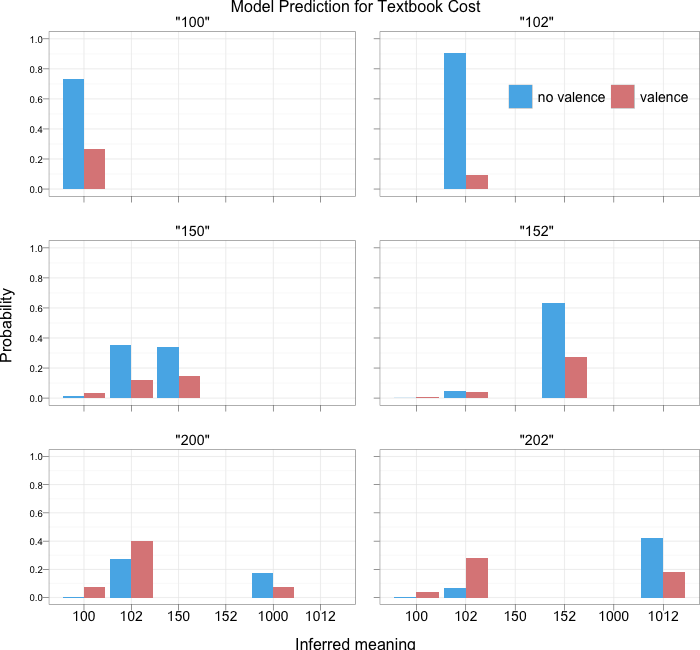
\includegraphics[width=\textwidth]{model_all_textbook.png}
%		\caption{model all textbook}
%	\end{subfigure}
%        \begin{subfigure}[b]{0.5\textwidth}
%                \centering
%                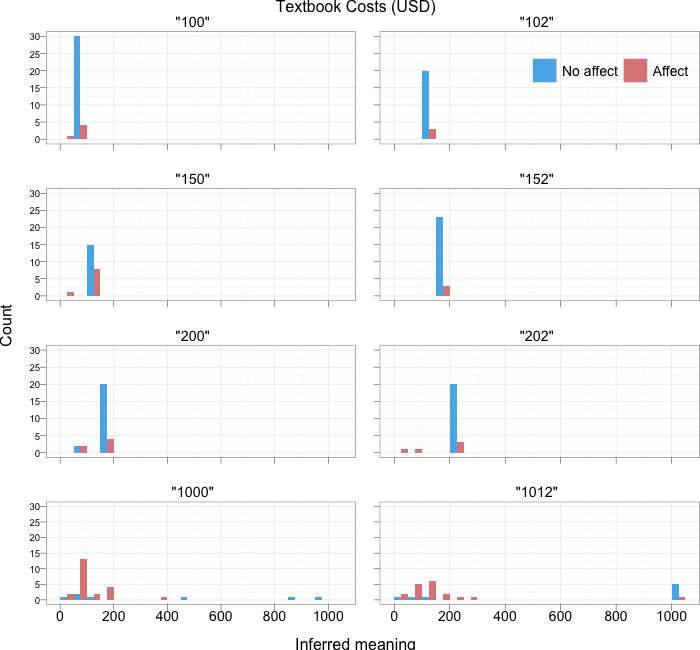
\includegraphics[width=\textwidth]{humans_all_textbook.png}
%		\caption{humans all textbook}
%	\end{subfigure}
%	\caption{The graph on the left shows rah rah rah and the one on the right shows roar roar roar}
%\end{figure}


\begin{figure}[t]
        \begin{subfigure}[b]{0.4\textwidth}
                \centering
                \caption{Pragmatic Halo}
		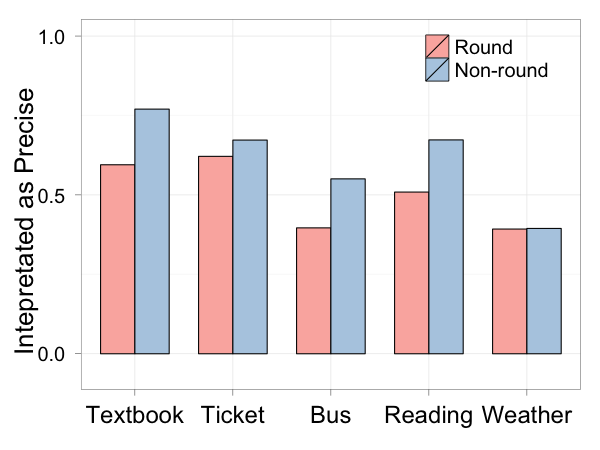
\includegraphics[width=\textwidth]{humans_halo_final.png}
		
	\end{subfigure} 
        \begin{subfigure}[b]{0.6\textwidth}
                \centering
                \caption{Exaggeration}
                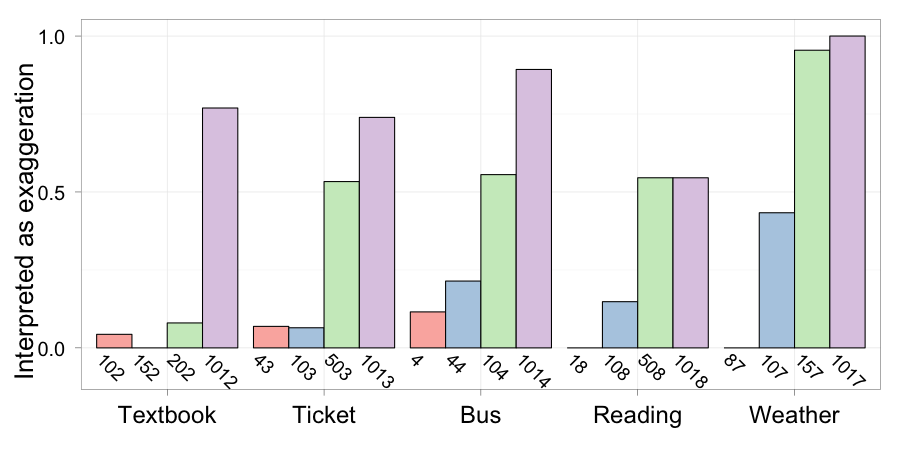
\includegraphics[width=\textwidth]{humans_exagg_all.png}
		
	\end{subfigure}
	\caption{Behavioral evidence for pragmatic halo and exaggeration effects across five scenarios}
	\label{fig:effects}
\end{figure}


\begin{figure}[H]
        \begin{subfigure}[b]{0.51\textwidth}
                \centering
                \caption{Model: Textbook costs}
                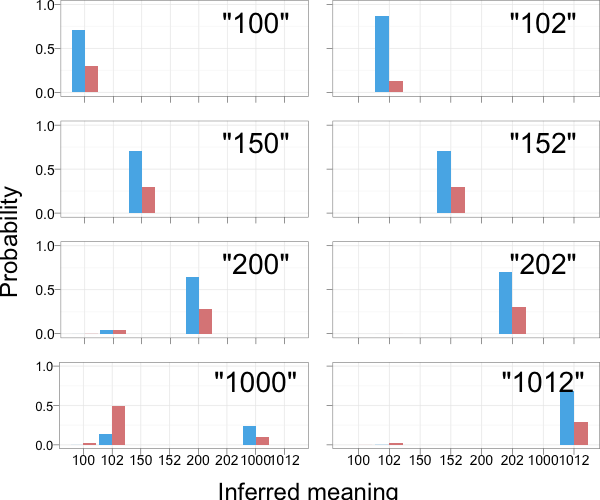
\includegraphics[width=\textwidth]{model_textbook_all.png}
	\end{subfigure}
        \begin{subfigure}[b]{0.51\textwidth}
                \centering
                \caption{Human: Textbook costs}
                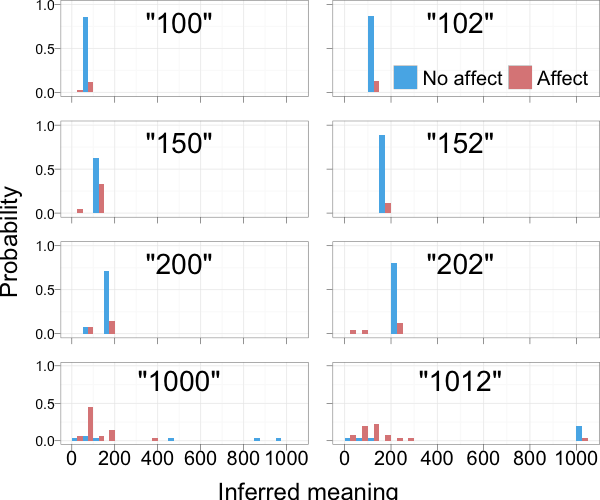
\includegraphics[width=\textwidth]{humans_textbook_all.png}
	\end{subfigure}
	\qquad
	
%\end{figure}
%\begin{figure}[t]
        \begin{subfigure}[b]{0.51\textwidth}
                \centering
                \caption{Model: Weather temperature}
                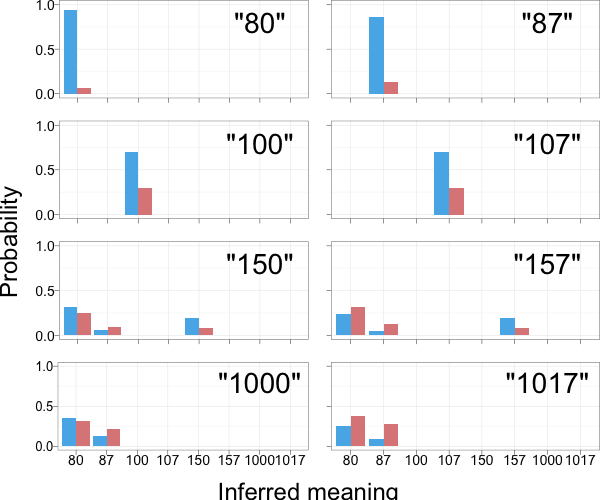
\includegraphics[width=\textwidth]{model_weather_all.png}
	\end{subfigure}
        \begin{subfigure}[b]{0.51\textwidth}
                \centering
                \caption{Humans: Weather temperature}
                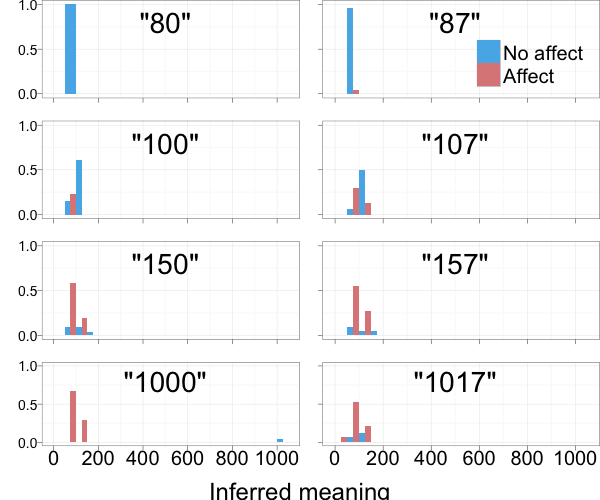
\includegraphics[width=\textwidth]{humans_weather_all.png}
        \end{subfigure}
	

        \qquad
        
%\end{figure}
%\begin{figure}[t]
       
       \begin{subfigure}[b]{0.51\textwidth}
                \centering
                \caption{Model: Length of reading}
                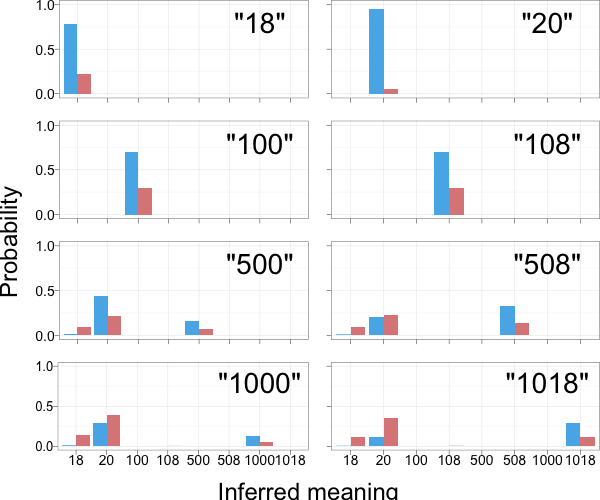
\includegraphics[width=\textwidth]{model_reading_all.png}
	\end{subfigure}
        \begin{subfigure}[b]{0.51\textwidth}
                \centering       
                \caption{Humans: Length of reading}         
                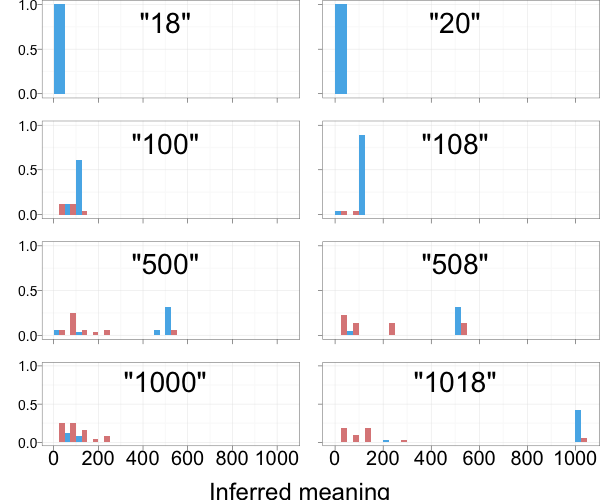
\includegraphics[width=\textwidth]{humans_reading_all.png}
        \end{subfigure} 
        \caption{Each row compares distributions of the model and subjects' interpretations of utterances. \textbf{Model:} Meaning prior $P(m) \propto b^m + c$  in all scenarios. For textbook costs, $(b, c) = (4 \times 10^4, 0.04)$; weather: $(b, c) = (2 \times 10^4, 0)$; reading length: $(b, c) = (8 \times 10^5, 0.04)$. Cost of round numbers is $0.25$; cost of non-round numbers is $0.286$. \textbf{Humans:} Subject's interpretations for each utterance are taken from Question (2) in Table 1. Interpretations are categorized as ``no affect" or ``affect" using a median split of subjects' responses to Question (3). Each bar indicates the probability of an utterance being interpreted as a certain meaning.}
        \label{fig:results}
  \end{figure}


%\subsubsection*{References}

\clearpage
\bibliographystyle{unsrt}
%\setlength{\bibleftmargin}{.125in}
%\setlength{\bibindent}{-\bibleftmargin}
%\bibnumfmt
\small{
\bibliography{nips_hyperbole}
}

\end{document}
